\section{Introduction}
With the rapid development of remote sensing technologies and popularization of geospatial related commercial software, high resolution satellite images are easily accessible. These valuable data provide a huge fuel for interpreting real terrestrial scenes. The building rooftop is one of the most important types of terrestrial objects because it is essential for a wide range of technologies, such as, urban planning, automated map making, 3D city modelling, disaster assessment, military reconnaissance, etc. However, it is very costly and time-consuming to manually delineate the footprint of buildings even for human experts. 

In recent decades, many researchers have made massive attempts to extract buildings automatically. Much of the past work defines criteria according to the particular  characteristics of rooftop, such as, polygonal boundary~\cite{noronha2001detection,nosrati2009novel,izadi2012three,wang2015efficient}, homogeneous color or texture~\cite{cote2013automatic}, surrounding shadow~\cite{B2008Building,ok2013automated,chen2014shadow,ngoautomatic}, and their combinations~\cite{baluyan2013novel,li2015robust}. However, such approaches are weakly capable of handling real-world data because hand-coded rules or probabilistic models learned from a small set of samples are heavily dependent on data. For example, they usually assume that the building rooftop is a polygon. However, stadiums typically have circle or oval shapes. Mnih~\cite{Mnih2013Machine} proposed a patch-based convolutional neural network to extract location of objects automatically and provided a huge public dataset including large-scale aerial images and their corresponding human-labeled maps. Based on Mnih's work, Saito \textit{et al}. improved the extraction accuracy further by developing new cost function and model averaging techniques~\cite{Saito2016Multiple}. Though these methods achieve high performance, they still have limited ability to deal with two frequently appearing cases: (1) buildings are occluded by shadows or trees and (2) buildings possess moderately variant appearances. 
% This paragraph should moved to the related work section. Why put it here? there are many algorithms to detect buildings. why only talk about the DNN approaches in the introduction section?  
%% Becuase DNN is our focus so we talk about it in detail.   

Extracting buildings from aerial image is essentially a problem of semantic segmentation. Recent work suggests a number of methods in processing natural images. Long \textit{et al.}~\cite{Long2014Fully} firstly proposed an effective architecture for semantic image segmentation, namely, fully convolutional network (FCN).
%   the coarse predictions from a late stage are upsampled and integrated with predictions from previous stage to yield finer ones, the whole procedure is repeated in this fashion until reaching a desired output. 
Chen \textit{et al.}~\cite{chen14semantic} presented a system which combines the responses at the final convolutional layer with a fully connected conditional random field (CRF). The system is able to accurately segment semantic objects. Zheng \textit{et al.}~\cite{Zheng2015Conditional} introduced an end-to-end network  which integrates CRF with CNNs to avoid off-line post-processing  for object delineation. Noh \textit{et al.}~\cite{Noh2015Learning} applied a deconvolution network to each proposal in an input image, and constructed the final semantic segmentation map by combining the results from all proposals.

%%%%%% introduce the difference of building extraction 

  Although these methods show good performance in natural image segmentation, they have components not suited for building extraction in aerial image in three aspects. 
	Firstly, each image in the PASCAL VOC 2012 dataset~\cite{pascal-voc-2012} has a handful of targets, while our source image is a complex scene, which has a number of targets with significant occlusions, variant appearances, and low contrast, as shown in Fig.~\ref{fig:AerialImages}(a)(b)(c), respectively. We directly integrate the coarse but strong semantic response into the output, instead of using CRF post-processing~\cite{Mnih2013Machine,chen14semantic}. 
	%Our network dramatically surpasses Mnih's~\cite{Mnih2013Machine} which has the same framework with DeepLab, so we advocate that CRF isn't the optimal choice in disposing complicated scenes. 
	Secondly, the image in our remote sensing dataset contains many tiny buildings, as Fig.~\ref{fig:AerialImages}(d) shows. Noh \textit{et al.}~\cite{Noh2015Learning} indicated that FCNs~\cite{Long2014Fully} have less abilities in processing small objects.	%while our network does pretty well in this case. They claimed their method handles objects in multiple scale, but it is only suitable to multi-classes object segmentation. 
	Thirdly, building extraction has much higher demand in precision of structure. The output of FCNs~\cite{Long2014Fully} has lower resolution which sacrifices precise structures severely.  
% (typically, $1/8$ of the resolution of the input image) 
\begin{figure}
	\centering
	\label{fig:AerialImages}
	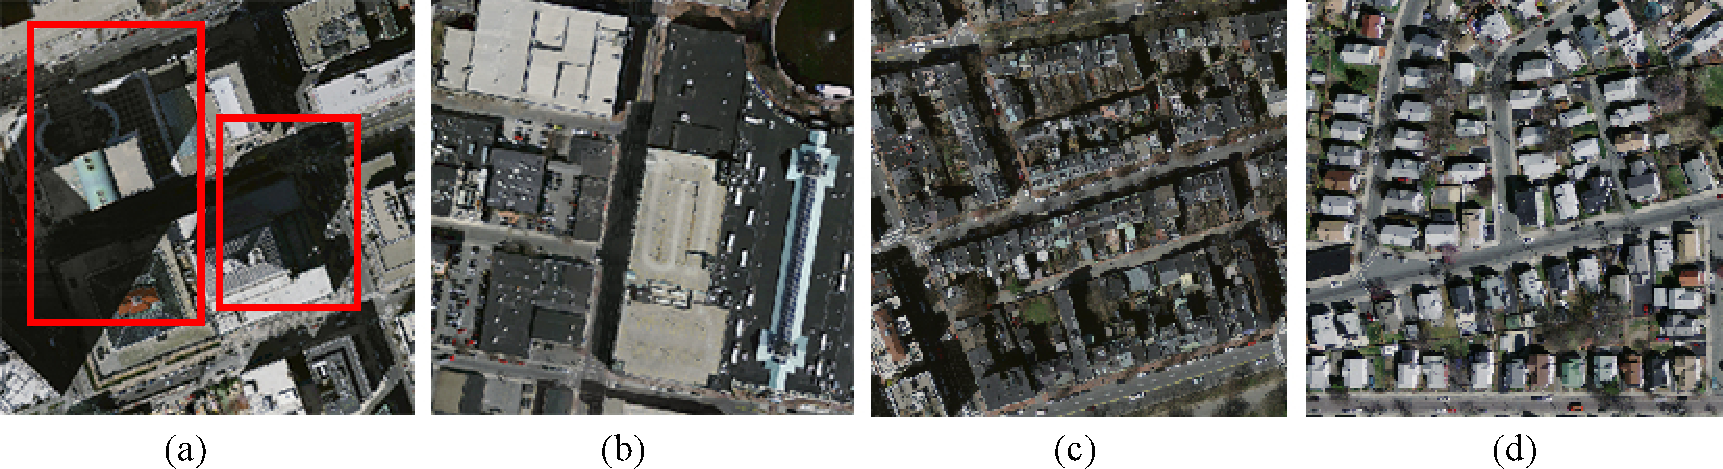
\includegraphics[width=120mm]{figs/AerialImages}
	\caption{Examples of aerial images with different type of challenges. (a) Occlusions in red boxes. (b) Variant appearances. (c) Low contrast. (d) A large number of tiny buildings. }
\end{figure}      

In this paper, we present a robust building extraction system by developing a hierarchically fused fully convolutional  network (HF-FCN). We trained our network on the large aerial image dataset~\cite{Mnih2013Machine}. In our architecture (HF-FCN), we design a new scheme to integrate multi-level semantic information generated from the convolutional layers with a group of increasing receptive fields, which capture context information of neighborhoods in different size. Therefore, it is more effective to handling buildings with arbitrary sizes, variant appearances or occlusions. Compared with the previous methods using convolution neural network \cite{Mnih2013Machine,Saito2016Multiple}, our HF-FCN does not require overlapped cropping and model averaging. Taking the whole image as input, it directly outputs the segmentation map by one pass of forward propagation. Therefore, the computational complexity is reduced significantly. In conclusion, our contributions include:
\begin{enumerate}
	\item A new architecture is developed for building extraction, which has a strong ability in processing appearance variations, varying building sizes and occlusions. The overall accuracy exceeds the state-of-the-art algorithms. 
	\item Our approach leads to a notable reduction of computation cost compared with previous solutions.
\end{enumerate}  

The rest of this article is organized as follows. In Section~\ref{section:relatedworks}, we summarize the related work for building extraction. Section~\ref{section:systemoverview} provides details of our neural network architecture. Section~\ref{section:experiments} introduces the dataset and training strategies of our proposed network, and experimental results while comparing our results to two state-of-the-art methods. 


\section{Related Work}
\label{section:relatedworks}
In previous studies, extracting buildings by employing their shape information is a dominant method. It is observed that rooftops have more regular shapes, which usually are rectangular or combinations of several rectangles. 
Several studies~\cite{noronha2001detection,nosrati2009novel,izadi2012three,wang2015efficient} exploited a graph-based search to establish a set of rooftop hypotheses through examining the relationship of lines and line intersections, and then removing the fake hypotheses using a series of manually designed criteria.
Cote and Saeedi~\cite{cote2013automatic} generated the rooftop outline from selected corners in multiple color and color-invariance spaces, further refine the outline by the level-set curve evolution algorithm. 
Though these methods based on geometric primitives achieved good performance in high contract remote sensing imagery, they suffer from three shortcomings. 
Firstly, they lack the ability of detecting arbitrarily shaped building rooftop. 
Secondly, they fail to  extract credible geometric features in buildings with inhomogeneous color distribution or low contrast with surroundings. 
Thirdly, it is time-consuming to process large-scale scenes because of their high computational complexity.	

Apart from using shape information, spectral information is a distinctive feature for terrestrial object extraction. For instance, shadows are commonly dark grey or black, vegetations are usually green or yellow with particular textures, and main roads are dim gray in most cases. According to these prior knowledge, Ghaffarian et al.~\cite{ghaffarian2014automaticPFICA} split aerial scenes into three components (respectively, shadows and the vegetation, roads and the bare soil, buildings) using a group of manually established rules. Afterwards, a purposive fast independent component analysis technique is employed to separate building area in remote sensing image. However, their results are significantly sensitive to parameter choice. A feasible alternative strategy is to learn the appearance representation using supervised learning algorithm~\cite{chen2014shadow,ngoautomatic,baluyan2013novel,dornaika2015object}. Firstly, an aerial image is divided into superpixels. Secondly, hand-crafted features, such as color histograms or local binary patterns, are extracted from each over-segmented region. Finally, each region is classified using machine learning tools and a gallery of training descriptors. Since it is inevitable for machine learning methods to mislabel regions with similar appearance, additional information is utilized to refine previous results. 
Ngo et al.~\cite{ngoautomatic} removed false rooftops using the assumption that buildings are surrounded by shadows because of illumination. Baluyan et al.~\cite{baluyan2013novel} devised a ``histogram method" to detect missed rooftops. Li et al.~\cite{li2015robust} selected probable rooftops after pruning out blobs using shadows, light direction, a series of shape criteria, and then these rooftops are refined by high order conditional random field. 
The drawbacks of these algorithms are threefold. 
(1) It is problematic to recognize an over-segmented region as building because terrestrial objects have hugely variant appearances in  real scene.
	(2) Hand-craft features are less expressive to tremendous shape or appearance difference of buildings. Therefore, it is not robust to process large-scale remote sensing images. 
(3) Additional information is unreliable in many cases. For instance, some low buildings have no shadow in its neighborhood, and many buildings have unique structures that do not satisfy the hand-coded criteria. 

As mentioned above, traditional methods are weakly capable of adapting to real scenes with huge variant appearances, occlusions or low contrast. 
%Our method does not rely on manually-designed image features. On the contrary, building features are directly learned from a mass of real data using deep neural networks. 
%Therefore, our algorithm is more robust to extract buildings in real scenes.  
Mnih, a pioneer, presented a patch-based framework for learning to label aerial images~\cite{Mnih2013Machine}. 
A neural network architecture is carefully designed for predicting buildings in aerial imagery, and the output of this network is processed by conditional random fields (CRFs). Satito \textit{et al.} \cite{Saito2016Multiple} improved Mnih's networks for extracting multiple kinds of objects simultaneously, two techniques consisting of model averaging with spatial displacement (MA) and channel-wise inhibited softmax (CIS) are introduced to enhance the  performance. However, these methods need to crop test image to a fixed size, which not only increases the time cost, but also breaks the integrity of buildings. Our system takes whole images as inputs without overlapped cropping or wrapping and directly outputs labelling images. It is much beneficial  to preserve the whole structure of buildings and shorten computation time.


%    For example, they obtain bad performance for large-size or occluded buildings (see Fig. \ref{fig:BadResults}) and cost about 9s for 1500 $\times$ 1500 image without model averaging. 

% Recently,  have been widely deployed in general image segmentation or scene labelling tasks.
